
\documentclass[12pt]{article}


\usepackage{times}
\usepackage{graphicx}
\graphicspath{{../local/}}
\usepackage{comment}
\usepackage{amsmath,amssymb}
\usepackage{natbib}

\usepackage{tikz}
\usetikzlibrary{arrows}



\topmargin 0.0cm
\oddsidemargin 0.2cm
\textwidth 16cm 
\textheight 21cm
\footskip 1.0cm



\newenvironment{sciabstract}{%
\begin{quote} \bf}
{\end{quote}}


\renewcommand\refname{References and Notes}


\newcounter{lastnote}
\newenvironment{scilastnote}{%
\setcounter{lastnote}{\value{enumiv}}%
\addtocounter{lastnote}{+1}%
\begin{list}%
{\arabic{lastnote}.}
{\setlength{\leftmargin}{.22in}}
{\setlength{\labelsep}{.5em}}}
{\end{list}}



\title{Disentangling sources of temporal clustering in intraspeaker variation using Generalized Additive Models} 



\begin{comment}
\author{Meredith Tamminga,$^{1\ast}$ Christopher Ahern,$^{1}$ Aaron Ecay$^{2}$\\
\\
\normalsize{$^{1}$Department of Linguistics, University of Pennsylvania}\\

\normalsize{$^{2}$Department of Language and Linguistic Science, University of York}\\
\\
\normalsize{$^\ast$To whom correspondence should be addressed: tamminga@ling.upenn.edu}}
\end{comment}

\author{}

\date{}



%%%%%%%%%%%%%%%%% END OF PREAMBLE %%%%%%%%%%%%%%%%



\begin{document} 


\baselineskip24pt


\maketitle 

\begin{abstract}
Intraspeaker variation is typically characterized by repetitiveness in variant choice, but there are multiple possible sources of such repetitiveness. We distinguish two types of clustering: sequential dependence, which we associate with priming, and baseline deflection, which we associate with style-shifting. We argue that because both priming and style-shifting are likely to be at play in producing observed quantitative patterns, it is desirable to adopt quantitative models that can simultaneously estimate sequential dependence and baseline deflection as distinct sources of temporal clustering. We propose the use of Generalized Additive Models (GAMs) for this purpose. We test the use of GAMs on a case study of DH-stopping in Philadelphia English sociolinguistic interviews and find that the resulting parameter estimates are reasonable given basic expectations about how style and priming should be distributed across individuals. We advocate for the adoption of this and similar new tools to advance the integration of psycholinguistic, sociolinguistic, and corpus linguistic insights in the study of intraspeaker variation.

\end{abstract}

\section{Introduction} \label{intro}


    
Non-independence of observations is a general problem in quantitative linguistic research \citep{paolillo:2002}. This is especially true for  research using naturalistic data that tries to connect observed variability in spontaneous speech with more carefully-controlled experimental results---connections which might serve both to confirm the real-world operation of psycholinguistic phenomena and to provide sociolinguists and corpus linguists with explanatory mechanisms for  observed patterns of variation. One source of non-independence is the collection of multiple data points per individual, which is of course necessary for the observation of intraspeaker variation. The introduction and uptake of mixed-effects regression \citep{Baayen:2008,Barr:2013} has allowed this type of non-independence to be controlled statistically. The collection of multiple observations from proximal locations is a similar problem in studies of spatially-distributed linguistic variation \citep{Wieling:2014}. In this paper we apply the same tool that has been used to handle geographic non-independence---Generalized Additive Models---to a problem of temporal non-independence: that sequential tokens of a varying linguistic item  in conversational speech are unlikely to be independent. Instead, temporally proximal instances of a variable are more likely to surface as the same variant \citep{Sankoff:1978}. 
    
We  distinguish two general classes of mechanisms that can give rise to such temporal clustering. First, there are what we term \textbf{sequential dependence} mechanisms: those in which the outcome of the variable in one moment influences the likelihood of a matching outcome some moments later. Intuitively, such a mechanism might be equated to \emph{priming} in the psycholinguistic sense, but we note that priming is itself potentially a cover term for a collection of facilitatory processes such as neural activation and implicit learning. Rather than taking a stance on the source of these processes, we adopt the terminology of sequential dependence to refer to any quantitatively-observed causal relationship between sequential instances of a variable.
    
The second source of temporal clustering is what \citet{Tamminga:2016a} call \textbf{externally-motivated baseline deflection}. If we imagine a speaker as having some target probability for production of a variable (a baseline), we might expect that target rate to fluctuate over time in response to elements in the real-world setting. Two closely-proximal instances of a variable are more likely to occur under similar circumstances than two instances that are further apart, and thus are more likely to be produced similarly. Just as sequential dependence as a term is intended to cover a range of possible factors, so too is the terminology of baseline deflection intended to capture many disparate elements of how speakers respond in real time to contextual and attitudinal factors, many of which have been discussed in sociolinguistics under the heading of \emph{style}. The social processes by which speakers dynamically situate themselves and their speech in a multidimensional space of social meaning are complex; the goal here is to reduce that information to a single abstract dimension in order to make it quantitatively tractable.


\begin{figure}
\begin{center}
        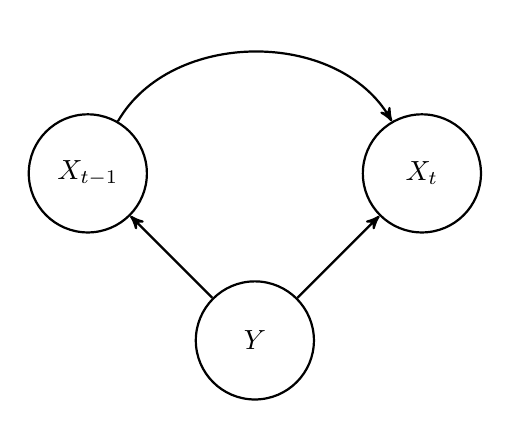
\begin{tikzpicture}[->,>=stealth',auto,node distance=3cm, thick]
	  \node (X) [draw,circle,minimum size=1.5cm]  at (0,0) {$X_{t-1}$};
	  \node (Z) [draw,circle,minimum size=1.5cm, below right of=X]  {$Y$};
	  \node (Y) [draw,circle,minimum size=1.5cm, above right of=Z]  {$X_{t}$};
	  \path[every node/.style={font=\sffamily\small}]
	    (Z) edge node [right] {} (X)
	    (Z) edge node [right] {} (Y)
	    (X) edge[bend left=60] node [right] {} (Y);
	\end{tikzpicture}         
    \end{center}
\caption{The relationship between sequential dependence and baseline deflections in the temporal use of variants}
\label{confounding}
\end{figure}

  
 In principle, sequential dependence and baseline deflection are distinct mechanisms. In practice, however, it has proven difficult to dissociate them in naturalistic data. Of particular consequence for research on intraspeaker variation in psycholinguistics is that this conflation leaves studies of priming in conversational speech vulnerable to the criticism that they are actually capturing something more like style-shifting or discourse coherence \citep{Szmrecsanyi:2006}. This problem can be summarized visually as in Figure \ref{confounding}, where we consider a sequence of tokens of a variable over time. We represent sequential dependence as an arrow from $X_{t-1}$ to $X_t$, indicating the influence of the previous outcome of the variable on the next outcome. We represent baseline deflections as an arrow from external factors $Y$ on the sequence of variants. In principle, we might conceive of baseline deflections as a confounding variable when it comes to estimating the effect of sequential dependence, or as sequential dependence as a confounding variable when it comes to estimating the effect of baseline deflections. However, given that we are interested in both aspects of variation, we need a means of estimating the two simultaneously.

 
 In this paper we propose the use of Generalized Additive Models (GAMs, \cite{hastie1990generalized}) for the simultaneous estimation of sequential dependence and baseline deflection.  GAMs allow for smooth functions of independent variables to be incorporated into models, which is ideal for modeling baseline deflection because for any given conversation, we have no \textit{a priori} expectations about when externally-motivated fluctuations in variant choice should occur. We use intraspeaker variation data drawn from a corpus of sociolinguistic interviews to illustrate this  application of GAMs. We include smooth functions of time elapsed in the models as a way of capturing baseline deflection in variant rates.  At the same time, we also include a predictor for the value of the previously-occurring token, which is the usual practice for identifying sequential dependence in sociolinguistic data: when prior use of a variant favors re-use of that variant, it is taken as evidence for priming. We suggest that using a GAM thus allows us to systematically attribute repetitiveness to either the value of the immediately prior token or overall fluctuations in variable rate due to contextual shifts. Further, we argue that in doing so, we end up with distributions of model estimates that are compatible with our expectations about how the plausible sources of sequential dependence (i.e. priming) and baseline deflections (i.e. style-shifting) should be distributed in populations, suggesting that this is a useful methodological approach for future research.
 

\section{Background}

The mechanisms of clustering that we term baseline deflection and sequential dependence are, as discussed above, most often thought to have their sources in sociolinguistically-meaningful speech style and psycholinguistic priming. Here we briefly outline the ways in which the temporal dynamics of style and priming have been addressed in the sociolinguistic and corpus linguistic literature.

\subsection{Style in sociolinguistics} \label{style}

Early work on speech style in sociolinguistics, particularly in the quantitative tradition exemplified by \citep{Labov:1966}, associated style-shifting with a single continuum: attention paid to speech. In this perspective, variables are seen as having vernacular and prestige variants, and when speakers attend consciously to their speech they move towards greater use of prestige variants across multiple variables at once. Stylistic analysis in this framework is  associated both with the deliberate manipulation of attention paid to speech, such as with reading passages, or with the use of heuristics such as \citet{Labov:2001}'s Style Decision Tree to code utterances for  aspects of the conversational context such as topic and interlocutor. Data aggregated within or (more often) across individuals is analyzed by way of these top-down categories; the analyst might ask questions like, ``Do speakers use more vernacular variants of this variable under conditions where they are distracted from monitoring their own speech?''. 

More recently, stylistic practice has come to the forefront of sociolinguistic theory \citep{Eckert:2012} (also see \citet{Eckert:2001} for an overview of various theories of style developed in the interim). What Eckert terms \emph{third wave sociolinguistics} focuses on how speakers dynamically deploy combinations of variants to position themselves socially, signal their stance toward the discourse, and generally express social meanings. \citet[3]{Podesva:2008} calls attention to the centrality of temporal dynamism in this view: ``Particular variants are unlikely to be randomly distributed over discourse; rather, if they have social meanings, they occur where their meanings are indexed in interaction.'' He calls for heightened methodological attention to the tricky task of ``representing how styles and their component linguistic features unfold over time'' \citeyearpar[6]{Podesva:2008}. The `variation scores' that Podesva develops are intended to be interpreted visually; howver, he notes that he has ``not yet developed a mathematical method for isolating [style] clusters'' \citeyearpar[7]{Podesva:2008}. This leaves open the possibility that apparent clusters are the outcome of chance variability rather than meaningful social practice. 

It is worthwhile to pursue novel methods used for analyzing style in variationist sociolinguistics because the current state of the art involves coding that is time intensive, subjective, and difficult to generalize. The analysis of linguistic style typically demands so much manual labor that the number of individual speakers studied is restricted. While this allows for nuanced portraits of individuals \citep{Podesva:2008,Johnstone:2006}, which are undoubtedly valuable in theorizing about style, it can limit the generalizability of the results. Relatedly, the sociolinguist analyzing style needs to make subjective decisions that substantially shape the results obtained. A different researcher with a different set of assumptions or priorities is likely to come to a very different set of conclusions.
Although stylistic practice is fundamentally tied to interactional moments in real time, the incorporation of temporal-sequential information into the analysis of style has lagged considerably behind the development of theories of social meaning. Even the best developed tools for studying the temporal dynamics of style in conversational speech, such as \citet{Podesva:2008}'s variation scores or Sharma and Rampton's Lectal Focusing in Interaction measure \citeyearpar{Sharma:2011}, provide descriptive quantitative characterizations of variant sequences but are unable to weigh in whether and how to attribute fluctuations in variant usage to externally motivated baseline deflections versus other sources, including sequential dependence.



\subsection{Priming in corpus data}

The study of style in sociolinguistic variation represents one perspective on why variants might cluster in speech. A second perspective is work on what is sometimes termed \emph{persistence} or \emph{priming} in conversational speech: the tendency to repeat a variant that has  recently been used. Research on corpus persistence comes from both  variationist sociolinguists   and  corpus linguists, with both traditions emphasizing the presumed connection between persistence as observed in conversational speech and priming as observed in the laboratory under carefully controlled experimental conditions \citep{Cameron:2004,Gries:2005,Szmrecsanyi:2006,Tamminga:2014b}.
In an experimental psycholinguistic context, priming may manifest as shortened reaction times for lexical access to primed words \citep{Goldinger:1996} or increased use of a primed syntactic structure in production \citep{Pickering:2008}. In naturalistic speech, the facilitation effects observed in the lab are arguably still at work, but identifying their effects is more difficult given the many factors at play in the production of conversational speech. Nonetheless, it has been argued that facilitation of variants equivalent to experimentally-induced priming emerges in the form of a recently-processed variant being more likely to reoccur than the alternative.

Besides the general level of noise and wide range of external factors in conversational speech, a specific concern in identifying the operation of priming in naturalistic data has been our inability to rule out stylistic clustering as an alternative source of apparent repetitiveness. Under a relatively simple conceptualization of style-shifting, the closer together two variable instances occur, the more likely they are to be co-located in a stylistically-coherent portion of the discourse and therefore the more likely they are to contain the same variant. It seems that more elaborate multi-variable and social-practice-based conceptualizations of style would make the same prediction. Externally-motivated baseline deflections thus have the potential to function as a confounding variable in observing relationships between primes and targets in conversational speech.

This tension between sequential dependence and baseline deflection has sometimes been framed in either--or terms. But the extensive evidence for both priming and style shifting independently suggests that multiple sources of repetitiveness may be at play simultaneously. The task, then, is not to adjudicate between style or priming (or similar mechanisms) as the better explanation for observed repetitiveness effects, but rather to estimate both of their effects independently.  
Doing so will allow us to strengthen the proposed link between corpus persistence and psychological priming effects as well as give statistical support to work on style.



\section{Estimating style and priming simultaneously}

We use Generalized Additive Models (GAMs) to simultaneously estimate sequential-dependent and baseline-deflective repetition in the socially-meaningful variation inherent to conversational speech. Our case study is a Philadelphia English sociolinguistic variable known as DH-stopping: the realization of the voiced interdental fricative as an apical stop or flap (informally, \emph{this} $\sim$ \emph{dis}, coded as $1$ and $0$ respectively; only word-initial DH-stopping is characteristic of Philadelphia English).  This variable is well suited to our purpose because it is stylistically dynamic \citep{Labov:2001}, and, being contained only in function words, unburdened by grammatical complications and highly  frequent in spontaneous speech. 

\subsection{Data}

The data we use are 18,022 observations of DH-stopping from 42 interviews with white working-class English speakers in the Philadelphia Neighborhood Corpus of sociolinguistic interviews \citep{Labov:2011a}.  The median number of observations per individual speaker is 367 (minimum 72, maximum 752). The interviews in the PNC have been transcribed and forced-aligned, facilitating auditory coding in Praat as described in \citet{Tamminga:2014b} (the original source of the data). While the realization of the voiced interdental fricative includes a range of phonetic variants over a mixture of closure and frication, the coding adopted here draws a binary distinction between tokens that do and do not exhibit some degree of frication, in line with Labov's assertion that only allophones lacking any frication are treated sociolinguistically as a meaningful variant \citep{Labov:2001a}.
\footnote{Many of the words that undergo to DH-stopping also have a pronunciation variant in which the interdental segment is entirely absent: \emph{'em} for \emph{them}. Following the original analysis of this data in \citet{Tamminga:2014b}, we exclude these occurrences on the grounds that they represent an independent historical development.} 

\subsection{Generalized Additive Models}

As we noted in Section \ref{style}, for any given speaker we have no \emph{a priori} expectation about what kind of baseline deflection would have been elicited by the discourse context in real time during the interview.  Whether a speaker style-shifts or not is dependent on many factors, most of which are properties of the real world social context and not readily accessible even via a transcript. Moreover, it is also the case that different speakers may engage in style-shifting to different degrees. Given that we lack knowledge about all of these external circumstances, GAMs are useful because they allow us to appropriately model this lack of knowledge. In other words, we adopt the GAM  as an elegant solution to treating time as a continuous variable in order to let the data ``speak for itself.'' \footnote{There are of course other methods that may yield similar results. For example, the use of \emph{Hidden Markov Models} to infer underlying states corresponding to styles by \citet{Ahern:2015} could be extended using \emph{Conditional Random Fields} to allow for the inference of both underlying states while also modeling the dependence between sequences of tokens.}


Using the \texttt{mgcv} package for the \texttt{R} statistical computing language \citep{R2015,wood2016}, we fit two logistic GAMs to each speaker's DH-stopping data: one with and one without a smooth function of time as a predictor. The more complex of the two models is as follows :
  
\begin{equation} \label{spline-mod}
  \text{DH-stopping variant} \hspace{12pt} \sim
  \underbrace{\text{s(time)}}_{\substack{\text{baseline deflection}}} 
  + \hspace{12pt} 
  \underbrace{\text{previous variant}}_{\text{sequential dependence}} \hspace{12pt} 
  * \hspace{12pt} 
  \underbrace{\text{ln(lag)}}_{\text{decay}}
  \vspace{12pt}
\end{equation}

In this model, we are predicting each observation of DH-stopping using: 1) a smooth function of time elapsed in the interview; 2) the outcome (observed variant) of the previous observation of the variable; 3) the time elapsed between the current and previous observation (which we refer to as the lag), log-transformed; and 4) the interaction of (2) and (3). The previous variant predictor plays the same role as it does in more traditional logistic regression models of priming in spontaneous speech: if facilitatory influence across sequential observations (intuitively, priming) is active, a previous stop variant is expected to decrease the likelihood of a fricative outcome in the current observation, while a previous fricative variant is expected to increase it. Including the interaction of the previous variant and the lag controls for the presumed decay over time of any potential priming effect. The smooth function of time is the component of the model  intended to capture baseline-deflective sources of repetitiveness (intuitively, style-shifting).


A smooth function in a GAM involves fitting a series of splines to the data at prespecified intervals, called knots, such that at each knot the regression spline on either side has the same value and first and second derivative. This leads to a curve that is smooth and continuous up to the second derivative but that has different shapes along the length of the curve. To avoid overfitting, the model fitting procedure assigns quadratic penalties for the regression splines in the maximum likelihood estimation.\footnote{See \cite{wood2006} for more detail on how penalized regression splines in GAMs work in principle and \cite{wood2016} for more detail on how they are implemented in \texttt{mgcv}.} 

If there is insufficient evidence for baseline deflection in the speaker's predicted rate of variant use over the course of the interview, the predicted time curve should be fairly linear as opposed to exhibiting more complex structure. In such a case the model in \eqref{spline-mod} should be comparable to a model that includes no smooth function of time---the simpler of the two models we fit to each speaker's data. We calculate the difference in Akaike Information Criteria (AIC, \cite{akaike1974}) between the two models (with and without the \emph{s(time)} term) for each speaker, adopting the rule of thumb that an AIC difference of less than 2 suggests that the more complex model is not an improvement over the simpler model \citep{burnham2003}. We use the results of the AIC comparison in the presentation below only to sort the speakers into those who do and don't exhibit substantial baseline deflections; in all cases we report the estimates from the full model.


\begin{figure}
    \centering
    \includegraphics[width=.7\textwidth]{style-speaker-LV.pdf}
    \caption{Predicted probability of use of fricative variant (\emph{this}) over course of interview.}
    \label{fig:style-speaker}
\end{figure}

Figure \ref{fig:style-speaker} shows the predicted values for a speaker who exhibits both sequential dependence and baseline deflection. Because the dependent variable is coded with the stop variant (\emph{dis}) as $0$, the y-axis is the predicted probability of a fricative variant (\emph{this}). The x-axis represents the time elapsed in the interview (in seconds). The reference level for the previous variant predictor is $1$: a prior observation in which the variant used is a fricative. The blue points representing observations for which the previous variant was a $1$, then, are higher than the red points because the speaker is more likely to re-use a recently-used variant. The dispersion of the red points results from the lag predictor controlling for the temporal decay of the sequential dependence effect. That the speaker exhibits baseline deflection can be seen in the fluctuations of the smooth line that the blue points approximate.


\subsection{Estimated parameters}


We begin by inspecting the previous variant estimates across the individual speakers' models (in Figure \ref{fig:style-speaker}, this would be the estimate of the vertical offset between the red and blue points). 
Three speakers are excluded because the models for their data failed to converge.
The resulting distribution of parameter estimates, each representing the operation of sequential dependence in a single speaker's DH-stopping data, is plotted in
Figure~\ref{fig:prime-dist}.
Sequential dependence, by virtue of its association with priming, is a source of clustering that we expect to characterize human cognition in general. We thus expect it to show a certain degree of homogeneity in the population, which is what we see in Figure \ref{fig:prime-dist}: though individual differences may exist, they do not divide the population into classes. 
Interestingly, we cannot reject the hypothesis that these estimates are normally distributed according to the \emph{Shapiro-Wilk test} ($W = 0.984$, $p = 0.830$). We suggest that the sequential dependence estimates reported here are  consistent with the assumption that priming is an automatic neural phenomenon underlying language production at a deep level. We take this as a preliminary indication that GAMs can be useful in identifying the operation of priming in naturalistic data.  

\begin{figure}
    \centering
    \includegraphics[width=.7\textwidth]{priming-density-LV.pdf}
    \caption{Distribution of logit priming coefficients in GAMs fit to 39 speakers} 
    \label{fig:prime-dist}
\end{figure}


Next, we turn to the baseline deflection components of the fitted models (in Figure \ref{fig:style-speaker}, the curve traced by the line of blue dots.
Each line in Figure \ref{wiggles} represents the smooth function of time as estimated for a single speaker, with the red lines on the left being speakers for whom the inclusion of the \emph{s(time)} term produced a change in AIC of less than 2 and the blue lines on the right being the speakers for whom the change in AIC is greater than 2. To examine the distribution of these lines in the sample population it would be useful to have a summary measure capturing the overall dynamism. For this purpose we adopt the estimated degrees of freedom contributed by the \emph{s(time)} term as a single-point metric of dynamism. The distribution of this metric across individuals is shown in Figure \ref{colorcurves}, which again is divided by speakers whose data are or are not better modeled by the more complex model.

\begin{figure}
    \centering
    \includegraphics[width=.7\textwidth]{dynamic-style-LV.pdf}
    \caption{Smooth functions of time in 39 individual speakers, faceted by $\Delta AIC < 2$ (Left) and $\Delta AIC > 2$ (Right)}
    \label{wiggles}
\end{figure}


\begin{figure}
    \centering
    \includegraphics[width=.7\textwidth]{edf-dynamic-LV.pdf}
    \caption{Estimated degrees of freedom contributed by \emph{s(time)} in 39 individual speakers, faceted by $\Delta AIC < 2$ (Left) and $\Delta AIC > 2$ (Right)}
    \label{colorcurves}
\end{figure}

The generalization we extract from the results in Figures \ref{wiggles} and \ref{colorcurves} is that the individual differences in baseline deflection are more robust than the individual differences in sequential dependence just discussed. 
These results are compatible with the view that baseline deflection reflects a causal mechanism, which we might loosely call  style-shifting, that is not an automatic process, but rather one over which speakers have some degree of control, albeit primarily subconscious. It is possible that the range of outcomes represents relatively uniform deployments of style-shifting behavior under widely differing contextual circumstances, but given that the conversational interactions are all sociolinguistic interviews on a predetermined set of topics, we doubt that this explanation would be sufficient to account for the individual differences. We suggest that different speakers have different degrees of dynamism in their sensitivity to context and attendant stylistic behavior, although of course it is likely that this is concurrent with contextual differences that could also produce some of the variability. In any case, that speakers exhibit widely divergent patterns of baseline deflection is consistent with the idea that we are capturing a context-dependent and speaker-controlled source of clustering with this component of the GAMs, in contrast to the homogeneity of sequential dependence.

\section{Discussion and directions} \label{discussion}

Generalized Additive Models can be used to simultaneously estimate two distinct sources of clustering in variant choice: sequential dependence and baseline deflection. The estimated distributions we presented in the previous section are encouraging in this respect: they accord with our prior expectations about how the causal forces producing these types of clustering should be distributed across individuals. The results that the models produce for these effects is consistent with an interpretation where sequential dependence is due to the automatic, universal process of priming and baseline deflection results from style-shifting in response to external contextual factors.


This paper is only a first step, which we hope may serve as an impetus for the development of this technique or the suggestion of alternative techniques for solving the same problem. 
There are a number of statistical issues that remain to be addressed in the use of GAMs for the purposes discussed here, including the choice of penalization scheme, the number and placement of knots, and basis splines. More generally, Generalized Additive Mixed Effects (GAMMs) offer a more robust means of dealing with variables that exhibit more complicated conditioning than DH-stopping while also improving statistical power in estimating effects.


Beyond refining the methodology of model specification and estimation, there are a number of future directions in which this work might be expanded. A natural question is whether the GAM results align with the results from top-down style-coding methods. In other words, do the peaks and dips of the fitted time curves line up in some way with the results of  manually coding the stylistic contexts in the same data? One way to operationalize this question would be to divide utterances into those for which the smooth function of time predicts the speaker is above or below their own grand mean, then compare utterance-by-utterance manual coding, for example as with Labov's \citeyearpar{Labov:2001} Style Decision Tree, to see if they agree on which utterances belong to high/formal and low/informal styles. If there is some reasonable amount of overlap between the output of the two methods, it would suggest that GAMs have promise as a method for automated style-coding, potentially reducing the amount of human labor involved in the analysis of style and thereby expanding the number of individuals who can be studied. 

Another avenue for future inquiry is that the model estimates differ across speakers, raising the possibility of relating individual differences in naturalistic behavior with individual differences in other cognitive or social properties of speakers. For example, it seems that only a minority of speakers show  significant baseline deflection in a sociolinguistic interview context: can we predict who these people are? Are there systematic correlations between the tendency to style shift and other sociolinguistically relevant factors, such as social network density or personality type? The method we have suggested here may thus be useful in tying conversational data to ongoing experimental work on individual differences in language variation and change \citep[inter alia]{Campbell-Kibler:2008,Baker:2011,Yu:2013,Forrest:2015} as well as in psycholinguistic laboratory behavior \citep[inter alia]{Stewart:2008,Dimov:2012,Lev-Ari:2014,Jun:2015}.

Finally, we are interested not only in applying this method to other types of variables but also in extending it to handle multiple variables at the same time. In the first case, we would like to investigate whether these patterns of sequential dependence and and baseline deflection are replicated with variables that differ from DH-stopping in their grammatical locus or sociolinguistic profile. Doing so may produce  new evidence pertaining to hypotheses about priming at different grammatical levels \citep{Tamminga:2014b} or to the availability of different variable types for stylistic practice \citep{Labov:1994}. Ultimately, though, the modern conception of speech style is one where variables crucially interact, motivating our desire to extend quantitative tools for the analysis of temporal dynamism in speech to the study of multiple variables at once.

The quantitative problem that we laid out at the beginning of this paper---multiple sources of repetitiveness---is one that has affected attempts to connect sociolinguistic and psycholinguistic research. While there is much work to be done in both the experimental and naturalistic empirical domains, a recurrent problem will be the need to develop new quantitative tools for analyzing the complexity of variation within and across individuals when all of the relevant factors are taken into account. It is our hope that the quantitative method we have suggested here can provide linguists from different traditions with a tool for unifying their perspectives.

%\bibliography{GAMpaper}

\bibliographystyle{apalike}





\end{document}